\section{Hardware Architecture}

\paragraph{}
The hardware platform chosen for this project is based on the Texas Instruments (TI) Sitara AM335x platform.
The AM335x series of System on a Chip (SoC) platform consists of an ARM Cortex-A8 processor running at up to 1 GHz as well as several other components <<am335x-overview>>.
The AM335x chip includes several built-in subsystems to meet the requirements of this project.
First, the platform is fully supported by the chosen bootloader and operating system.
Second, the platform contains the necessary interfaces and components to integrate and support any external peripheral devices required by the project.
Finally, the SoC is community-backed with cheap single-board computer implementations such as the BeagleBone Black (BBB).
The BBB was chosen as the basis of this project's hardware reference platform due to its reasonable cost and versatility.

\subsection{Computing}

\paragraph{}
The AM335x includes an ARM CPU with adequate processing power for this project.
The CPU can run as fast as 1 GHz and has mature support within u-boot and Linux.
Since Linux is not a Real Time Operating System (RTOS), there are use cases where Linux cannot be relied upon.
For these cases, Linux can work cooperatively with two additional built-in processors, the TI PRUSS units which are RISC processors that run at 200MHz and are fully programmable.

\subsection{Graphics}

\paragraph{}
The AM335x platform contains its own Graphics Processing Unit (GPU).
The main purposes of this GPU are for hardware-accelerated 3D graphics and video playback.
These features are not necessary for this project but may be useful in the future.
The project still requires the display of two-dimensional graphics, however.
The AM335x contains a framebuffer unit which supports LCD as well as HDMI video output.
This framebuffer is supported by the X11 window manager as well as other Linux-compatible graphics systems.
For the display component, a 3.5" TFT display was chosen.

\subsection{Audio}

\paragraph{}
The AM335x platform contains 2 dedicated TI McASP (Multi-channel Audio Serial Port) audio processing units which are capable of supplying audio data from the system to connected audio codec chips.
The McASP supports transmitting and receiving digital audio signals in I2S as well as PCM and S/PDIF formats to codec chips.
The TI PCM5102 I2S DAC codec was chosen for this project, simply because it requires little configuration and has several break-out boards that are easy to obtain and inexpensive.
Each codec board supports two channel output so it is necessary to integrate two codecs with the McASP.
The I2S audio protocol packs two channels of audio into a single data line, switching between them using a frame-sync clock.
Each McASP unit has four data lines (serializers) so the first two are connected to each codec's data input port.
Each codec will also receive two clock signals from the McASP, the bit clock and the frame-sync clock.
The bit clock is a clock signal which is used to time the audio data emitted by the serial port and has a timing always a multiple of the frame sync clock.
These signals are shared across the entire I2S bus controlled by the McASP.
In this configuration (Figure ~\ref{fig:audio-circuit-i2s}), the McASP is considered the master and both codecs are considered slaves.
The I2S specification also calls for a high-speed clock, also called the master clock, which typically is divided to derive the other clocks, though the PCM5102 does not need this signal.

\begin{figure}
  \centering
  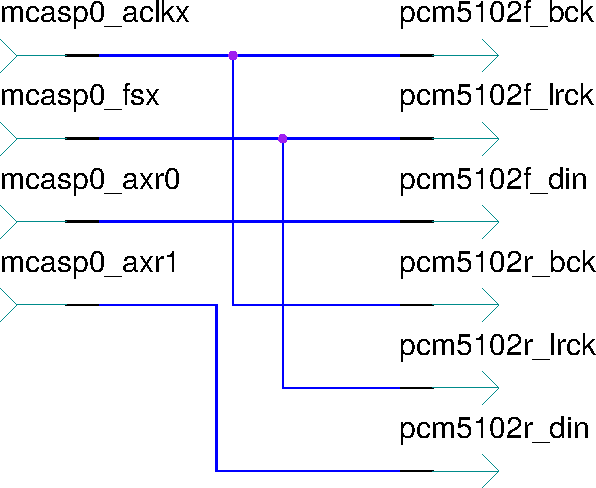
\includegraphics[width=0.65\textwidth,page=1]{audio-circuit-i2s}
  \caption{I2S audio configuration (power not shown)}
  \label{fig:audio-circuit-i2s}
\end{figure}

\subsection{Storage}

\paragraph{}
The AM335x platform allows several options for storage.
It has built-in controllers for MMC, NAND, and NOR flash memory.
Other storage can also be added over its USB interfaces.
The BBB includes an embedded MMC (eMMC) storage unit which will be used to store the operating system including the bootloader, kernel, and root filesystem.
The USB interface support will allow external storage devices to supply data to the system such as music files and geographical information.

\subsection{Peripheral Buses}

\paragraph{}
In addition to the previously mentioned buses, the AM335x platform contains controllers for several other, more general purpose communications buses.
It has controllers for I2C, SPI, and UART serial interfaces.
These controllers can be used to connect the host system to a range of peripherals such as GPS receivers, terrestrial radio receivers, as well as wireless network interfaces such as 802.11 and Bluetooth.
As previously mentioned, USB is also available as a general purpose peripheral bus.

\subsection{Bluetooth Networking}

\paragraph{}
For Bluetooth networking, a commodity USB bluetooth adapter has been selected for this project based on the CSR8510 chipset.

\subsection{802.11 Networking}

\paragraph{}
For 802.11 wireless networking, a commodity USB 802.11n adapter bas been selected for this project based on the MT7601 chipset.

\subsection{Touchscreen}

\paragraph{}
For the touchscreen input, a screen with the XPT2046 controller was chosen.
This controller communicates with the host over SPI and is packaged with the chosen TFT display.

\subsection{GPS}

\paragraph{}
In order to provide location information, the hardware reference platform includes a GPS receiver module.
This module is connected to the host over the UART serial interface, using 3 signalling pins and a power connection (Figure ~\ref{fig:gps-circuit-uart}).
GPS data is emitted by the transmit pin of the GPS module into the receive pin of the host and a clock signal is emitted by the PPS signal of the GPS module into the carrier detect pin of the host.
The GPS module chosen for this project is a MT3339 chipset inside a GlobalTop FGPMMOPA6C self-contained module.

\begin{figure}
  \centering
  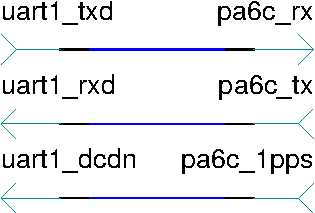
\includegraphics[page=1]{gps-circuit-uart}
  \caption{GPS serial connection (power not shown)}
  \label{fig:gps-circuit-uart}
\end{figure}

\subsection{Other Pins}

\paragraph{}
The AM335x platform also contains several general-purpose pins which can be used for less complex operations than typical peripheral bus protocols such as indicator circuits and as a host interrupt source.
These extra pins are also used to supplement functionality of devices connected over another bus such as SPI or MMC.
In addition, the AM335x platform also includes support for pulse-width modulation (PWM) input and output, which can be used to drive clock signals, some types of motors, and dimmable LED light sources as well as the capture of the input source intensity.
